% Generated by render.py; edit preamble.tex, citations.json and main.tikz
\documentclass[border=12pt]{standalone}
\def\pgfsysdriver{pgfsys-dvisvgm.def}
\usepackage[dvisvgm]{xcolor}
\usepackage{xeCJK}
\setCJKmainfont{HaranoAjiGothic-Regular.otf}[BoldFont=HaranoAjiGothic-Bold.otf]
\setCJKsansfont{HaranoAjiGothic-Regular.otf}[BoldFont=HaranoAjiGothic-Bold.otf]
\usepackage{amsmath,amssymb,tikz,lmodern}
\usetikzlibrary{arrows.meta,positioning,calc,fit,backgrounds}
\renewcommand{\familydefault}{\sfdefault}
\definecolor{ink}{HTML}{25322F}
\definecolor{green}{HTML}{246657}
\definecolor{tint}{HTML}{EEF4F0}
\definecolor{soft}{HTML}{C6D2CC}
\definecolor{muted}{HTML}{52615B}
\newif\ifJapanese
\newcommand{\Tx}[2]{\ifJapanese #1\else #2\fi}
\newcommand{\Eff}{\overline{\operatorname{Eff}}}
\newcommand{\heading}[3]{{\color{green}\bfseries #1\quad\Tx{#2}{#3}}\\[5pt]}
% A white rectangle makes the complete citation label clickable, including spaces.
\newcommand{\refurl}[2]{\special{dvisvgm:raw <a xlink:href="#1" target="_blank" rel="noopener noreferrer">}{\setlength{\fboxsep}{0pt}\colorbox{white}{\color{green}\underline{\strut #2}}}\special{dvisvgm:raw </a>}}
\tikzset{
 card/.style={draw=soft,fill=white,rounded corners=2pt,align=left,text=ink,font=\fontsize{10.5}{14}\selectfont,inner xsep=12pt,inner ysep=10pt,text width=14.4cm},
 half/.style={card,text width=6.45cm,minimum height=2.05cm},
 result/.style={card,draw=green,fill=tint,line width=.9pt},
 reason/.style={align=left,text=muted,font=\fontsize{9}{12}\selectfont,inner sep=0pt,text width=12.6cm},
 branchreason/.style={reason,text width=5.95cm},
 edge/.style={-{Stealth[length=2.4mm]},draw=green,line width=1pt},
 wire/.style={draw=green,line width=1pt},
}
% Keep the arrow in a dedicated left gutter; explanations never cover it.
\def\flow#1#2#3;{
 \coordinate (#2-from) at ($(#1.south)+(-6.9,0)$);
 \coordinate (#2-to) at ($(#2.north)+(-6.9,0)$);
 \draw[edge] (#2-from)--(#2-to);
 \node[reason,anchor=west] (#2-reason) at ($(#2-from)!.5!(#2-to)+(.55,0)$) {#3};
}

% Style adapted from the repository's Schnell diagrams; MIT attribution retained.

% Generated from citations.json; do not edit.
\newcommand{\Cite}[1]{\csname cite-#1\endcsname}
\expandafter\def\csname cite-main-result\endcsname{\shortstack[l]{\refurl{https://github.com/openai/math/blob/1581d4cbdd69a0faf34b2089614fe2a814316a6a/preprints/Nagatas-Conjecture-for-Plane-Curves-September-23-2026/main.pdf}{Theorem 1.1 · p. 1}}}
\expandafter\def\csname cite-fields\endcsname{\shortstack[l]{\refurl{https://github.com/openai/math/blob/1581d4cbdd69a0faf34b2089614fe2a814316a6a/preprints/Nagatas-Conjecture-for-Plane-Curves-September-23-2026/main.pdf}{Corollary 6.1 · p. 22}}}
\expandafter\def\csname cite-positivity\endcsname{\shortstack[l]{\refurl{https://github.com/openai/math/blob/1581d4cbdd69a0faf34b2089614fe2a814316a6a/preprints/Nagatas-Conjecture-for-Plane-Curves-September-23-2026/main.pdf}{Corollary 6.2 · p. 22}}}
\expandafter\def\csname cite-universal\endcsname{\shortstack[l]{\refurl{https://github.com/openai/math/blob/1581d4cbdd69a0faf34b2089614fe2a814316a6a/preprints/Nagatas-Conjecture-for-Plane-Curves-September-23-2026/main.pdf}{Lemma 2.1 · pp. 3–4}}}
\expandafter\def\csname cite-normal\endcsname{\shortstack[l]{\refurl{https://github.com/openai/math/blob/1581d4cbdd69a0faf34b2089614fe2a814316a6a/preprints/Nagatas-Conjecture-for-Plane-Curves-September-23-2026/main.pdf}{Proposition 2.2 · pp. 4–6}}}
\expandafter\def\csname cite-square\endcsname{\shortstack[l]{\refurl{https://github.com/openai/math/blob/1581d4cbdd69a0faf34b2089614fe2a814316a6a/preprints/Nagatas-Conjecture-for-Plane-Curves-September-23-2026/main.pdf}{Proposition 2.3 · pp. 6–7}}}
\expandafter\def\csname cite-cubic\endcsname{\shortstack[l]{\refurl{https://github.com/openai/math/blob/1581d4cbdd69a0faf34b2089614fe2a814316a6a/preprints/Nagatas-Conjecture-for-Plane-Curves-September-23-2026/main.pdf}{Lemma 2.4; Proposition 3.1 · pp. 8–9}}}
\expandafter\def\csname cite-theta\endcsname{\shortstack[l]{\refurl{https://github.com/openai/math/blob/1581d4cbdd69a0faf34b2089614fe2a814316a6a/preprints/Nagatas-Conjecture-for-Plane-Curves-September-23-2026/main.pdf}{Lemmas 3.2–3.3; §3.3 · pp. 10–12}}}
\expandafter\def\csname cite-collision\endcsname{\shortstack[l]{\refurl{https://github.com/openai/math/blob/1581d4cbdd69a0faf34b2089614fe2a814316a6a/preprints/Nagatas-Conjecture-for-Plane-Curves-September-23-2026/main.pdf}{Lemma 4.1 · pp. 13–14}}}
\expandafter\def\csname cite-matrix\endcsname{\shortstack[l]{\refurl{https://github.com/openai/math/blob/1581d4cbdd69a0faf34b2089614fe2a814316a6a/preprints/Nagatas-Conjecture-for-Plane-Curves-September-23-2026/main.pdf}{Lemma 4.2; Proposition 4.3 · pp. 14–17}}}
\expandafter\def\csname cite-rows\endcsname{\shortstack[l]{\refurl{https://github.com/openai/math/blob/1581d4cbdd69a0faf34b2089614fe2a814316a6a/preprints/Nagatas-Conjecture-for-Plane-Curves-September-23-2026/main.pdf}{Lemmas 5.1–5.4 · pp. 18–21}}}
\expandafter\def\csname cite-full-rank\endcsname{\shortstack[l]{\refurl{https://github.com/openai/math/blob/1581d4cbdd69a0faf34b2089614fe2a814316a6a/preprints/Nagatas-Conjecture-for-Plane-Curves-September-23-2026/main.pdf}{Proposition 5.5; Theorem 1.1 proof · p. 21}}}
\expandafter\def\csname cite-reading-scope\endcsname{\shortstack[l]{\refurl{https://github.com/openai/math/blob/1581d4cbdd69a0faf34b2089614fe2a814316a6a/preprints/Nagatas-Conjecture-for-Plane-Curves-September-23-2026/main.pdf}{§§2–6 · pp. 3–22}}}
\expandafter\def\csname cite-normal-input\endcsname{\shortstack[l]{\refurl{https://stacks.math.columbia.edu/download/divisors.pdf\string##page=26}{[StacksN, Tag 0B3P, Lemma 15.2, p. 26]}}}
\expandafter\def\csname cite-cohomology-input\endcsname{\shortstack[l]{\refurl{https://stacks.math.columbia.edu/download/coherent.pdf\string##page=16}{[StacksC, Tag 01XT, Lemma 8.1, p. 16]}}}
\expandafter\def\csname cite-torsion-input\endcsname{\shortstack[l]{\refurl{https://stacks.math.columbia.edu/download/curves.pdf\string##page=36}{[StacksT, Tag 0C1Z, Lemma 17.1, p. 36]}}}

\Japanesetrue
\begin{document}
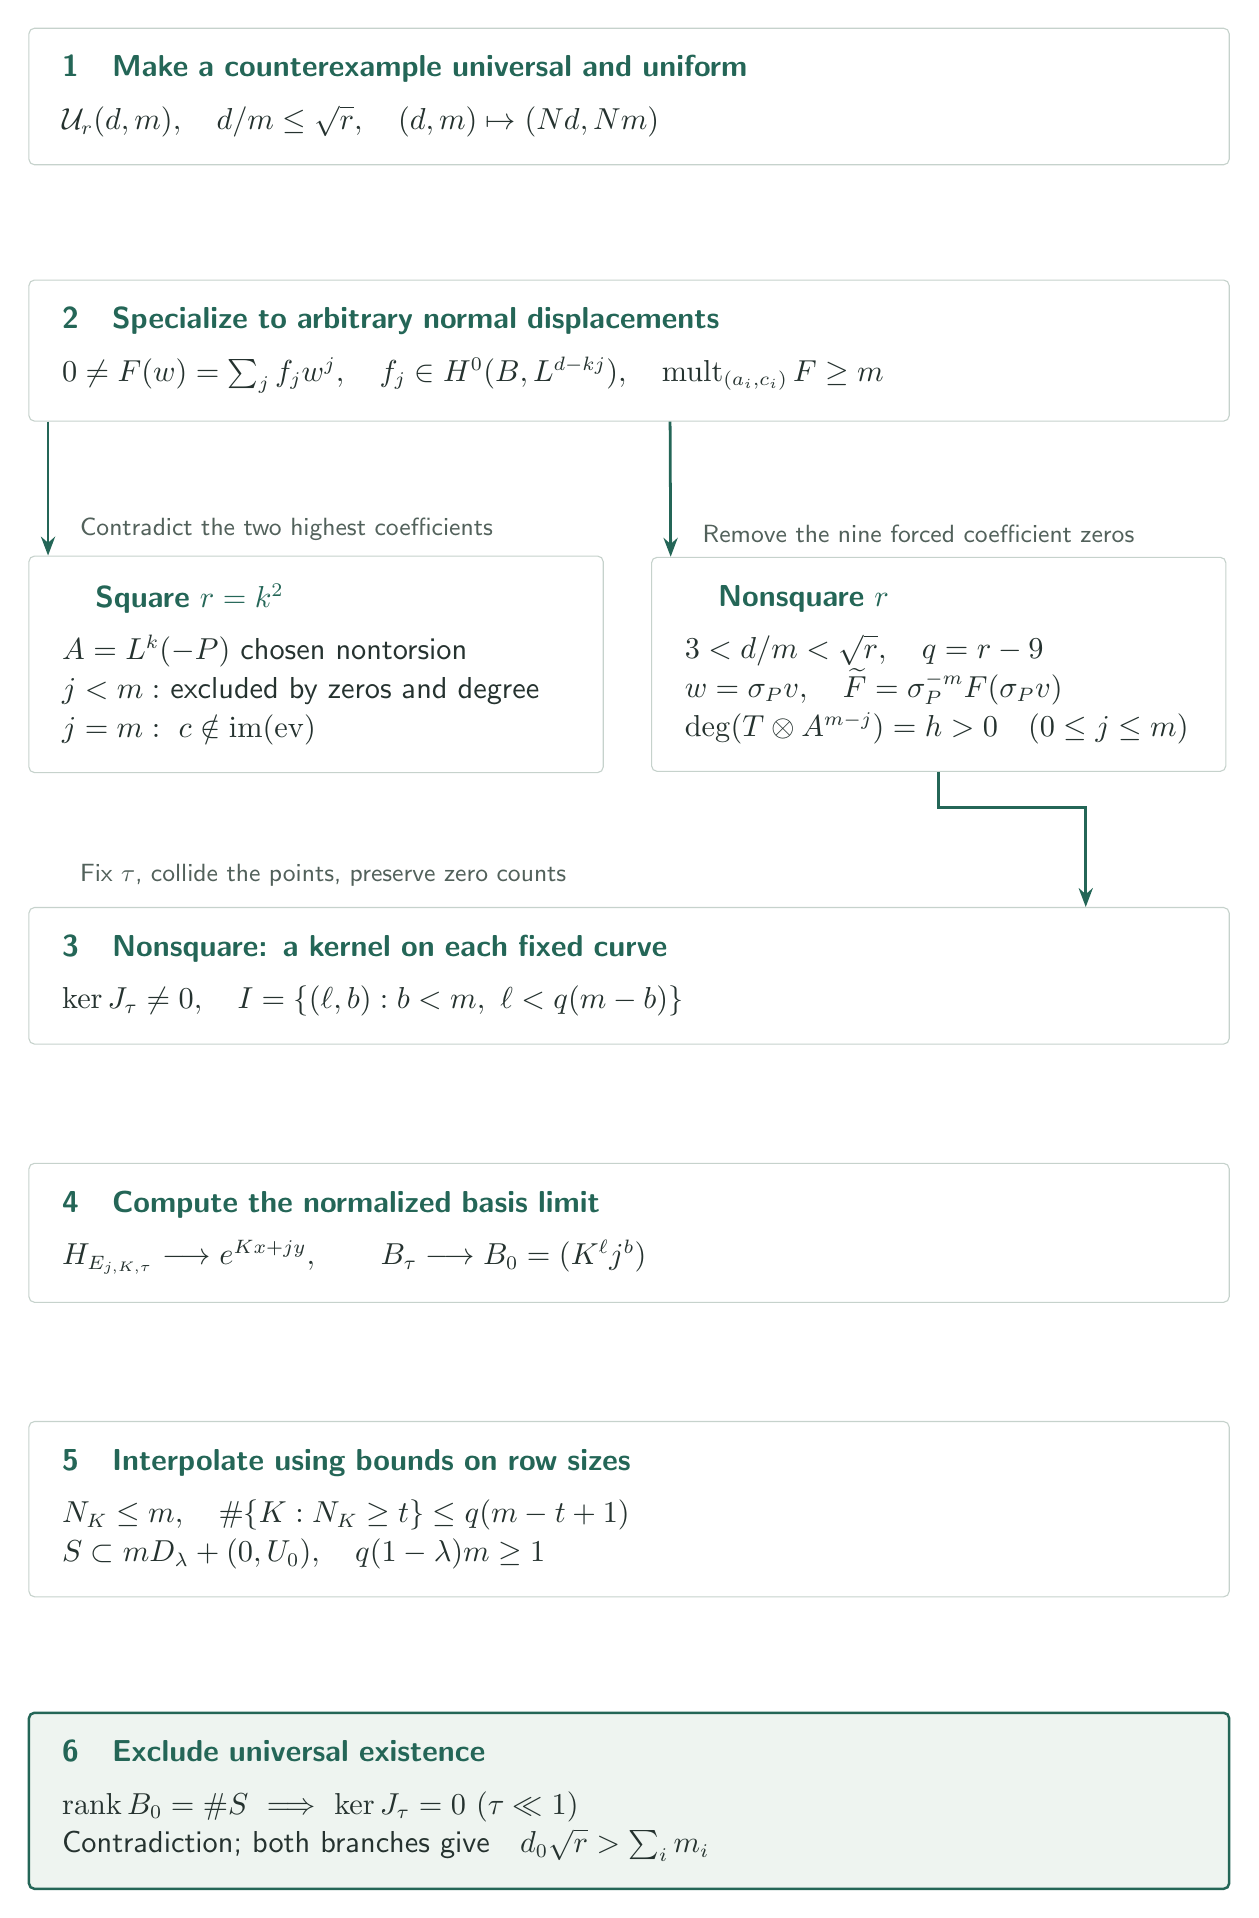
\begin{tikzpicture}
\node[card] (a) {\heading{1}{反例を全配置の均等系へ}{Make a counterexample universal and uniform}
$\mathcal U_r(d,m),\quad d/m\le\sqrt r,\quad (d,m)\mapsto(Nd,Nm)$};
\node[card,below=1.45cm of a] (b) {\heading{2}{任意の法変位へ特殊化}{Specialize to arbitrary normal displacements}
$0\ne F(w)=\sum_j f_jw^j,\quad f_j\in H^0(B,L^{d-kj}),\quad \operatorname{mult}_{(a_i,c_i)}F\ge m$};
\flow a b {\Tx{閉 incidence 条件と巡回積、法座標の拡大}{Closed incidence conditions, cyclic products, rescaled normal coordinate}\\\Cite{universal};\quad\Cite{normal}};
\node[half,below=1.7cm of b.south west,anchor=north west] (sq) {\heading{}{平方 $r=k^2$}{Square $r=k^2$}
$A=L^k(-P)$ \Tx{を非捩れに選ぶ}{chosen nontorsion}\\
$j<m:$ \Tx{零点数と次数で排除}{excluded by zeros and degree}\\
$j=m:\ c\notin\operatorname{im}(\mathrm{ev})$};
\node[half,right=.6cm of sq] (ns) {\heading{}{非平方 $r$}{Nonsquare $r$}
$3<d/m<\sqrt r,\quad q=r-9$\\
$w=\sigma_Pv,\quad\widetilde F=\sigma_P^{-m}F(\sigma_Pv)$\\
$\deg(T\otimes A^{m-j})=h>0\quad(0\le j\le m)$};
\draw[edge] ($(b.south west)+(.25,0)$)--($(sq.north west)+(.25,0)$);
\draw[edge] ($(b.south west)+(8.15,0)$)--($(ns.north west)+(.25,0)$);
\node[branchreason,anchor=south west] at ($(sq.north west)+(.65,.18)$) {\Tx{二つの最高係数で矛盾}{Contradict the two highest coefficients}\\\Cite{square}};
\node[branchreason,anchor=south west] at ($(ns.north west)+(.65,.18)$) {\Tx{九点の強制零点を除く}{Remove the nine forced coefficient zeros}\\\Cite{cubic}};
\node[card,below=1.7cm of sq.south west,anchor=north west] (c) {\heading{3}{非平方：各曲線上で非零核を得る}{Nonsquare: a kernel on each fixed curve}
$\ker J_\tau\ne0,\quad I=\{(\ell,b):b<m,\ \ell<q(m-b)\}$};
\draw[edge] (ns.south)--($(ns.south)+(0,-.45)$)-|($(c.north)+(5.8,0)$);
\node[reason,anchor=south west] at ($(c.north west)+(.65,.25)$) {\Tx{$\tau$ を固定して点を衝突、零点数を保存}{Fix $\tau$, collide the points, preserve zero counts}\\\Cite{collision}};
\node[card,below=1.5cm of c] (d) {\heading{4}{正規化基底の極限を計算}{Compute the normalized basis limit}
$H_{E_{j,K,\tau}}\longrightarrow e^{Kx+jy},\qquad B_\tau\longrightarrow B_0=(K^\ell j^b)$};
\flow c d {\Tx{theta 級数の全固定階微分が収束}{Theta series converge with every fixed derivative}\\\Cite{matrix}};
\node[card,below=1.5cm of d] (e) {\heading{5}{行の個数を制御して補間}{Interpolate using bounds on row sizes}
$N_K\le m,\quad\#\{K:N_K\ge t\}\le q(m-t+1)$\\
$S\subset mD_\lambda+(0,U_0),\quad q(1-\lambda)m\ge1$};
\flow d e {\Tx{縮小多角形と共通倍で格子端点誤差を吸収}{A contracted polygon and common powers absorb endpoint errors}\\\Cite{rows}};
\node[result,below=1.45cm of e] (f) {\heading{6}{全配置の存在を排除する}{Exclude universal existence}
$\operatorname{rank}B_0=\#S\ \Longrightarrow\ \ker J_\tau=0\ (\tau\ll1)$\\
\Tx{非零核と矛盾し、平方・非平方とも}{Contradiction; both branches give}\quad $d_0\sqrt r>\sum_i m_i$};
\flow e f {\Tx{行補間の全射性と非零小行列式の持続}{Surjective row interpolation and persistence of a nonzero minor}\\\Cite{full-rank}};

\end{tikzpicture}
\end{document}
